\subsection{Caso d'uso UC9: Modifica della presentazione}
\begin{figure}[h] 
	\centering 
	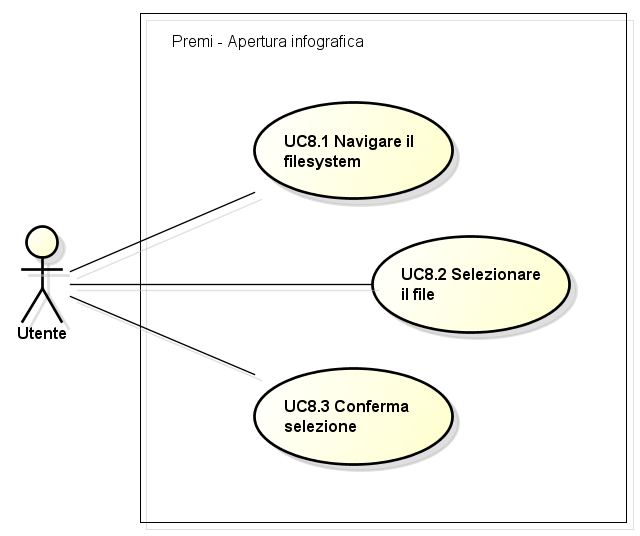
\includegraphics[scale=0.3] {img/UC9.png}
	\caption{UC9 - Modifica della presentazione} 
\end{figure}

\begin{itemize}
	\item \textbf{Attori:} Proprietario;
	\item \textbf{Scopo e descrizione:} L'utente sta lavorando su una presentazione per inserire delle nuove \gls{slide} o per modificare quelle già create. Può quindi inserire  elementi come: \gls{slide}, immagini, caselle di testo e dati \gls{real time}. Ha inoltre la possibilità di modificare gli elementi già inseriti, oppure di eliminarli. Può infine scegliere l'effetto di transizione tra una \gls{slide} e l'altra;
	\item \textbf{Precondizione:} L'utente ha creato una nuova presentazione nella fase di creazione di un progetto o ha aperto un progetto creato in precedenza per modificarlo;
	\item \textbf{Flusso principale degli eventi:}
	\begin{enumerate}
		\item L'utente sceglie il \gls{template} [UC9.1];
		
		\item L'utente inserisce una nuova \gls{slide} [UC9.2];
		
		\item L'utente rimuove una \gls{slide} [UC9.3];
		
		\item L'utente inserisce un'immagine [UC9.4];
		
		\item L'utente inserisce una casella di testo [UC9.5];
		
		\item L'utente inserisce dati \gls{real time} [UC9.6];
		
		\item L'utente inserisce una tabella [UC9.7];
		
		\item L'utente inserisce un grafico [UC9.8];
		
		\item L'utente sceglie un effetto di transizione [UC9.9];
		
		\item L'utente cambia la dimensione di un elemento [UC9.10];
		
		\item L'utente cambia la posizione di un elemento [UC9.11];
		
		\item L'utente ruota un elemento [UC9.12];
		
		\item L'utente rimuove un elemento [UC9.13];

		\item L'utente carica un file per inserire l'immagine [UC9.14];

		\item L'utente sceglie la formattazione del testo [UC9.15];

		\item L'utente modifica una tabella [UC9.16];

		\item L'utente modifica un grafico [UC9.17];
		
		\item L'utente inserisce note/parole chiave [UC9.18];
		
		\item L'utente sposta una \gls{slide} [UC9.19].
	\end{enumerate}
	\item \textbf{Postcondizione:} Il sistema esegue le operazioni effettuate dall'utente.
\end{itemize}


\subsection{Caso d'uso UC9.1: Scegliere un template}
\begin{itemize}
	\item \textbf{Attori:} Proprietario;
	\item \textbf{Scopo e descrizione:} L'utente sceglie un \gls{template} di stile da utilizzare per la propria presentazione;
	\item \textbf{Precondizione:} L'utente sta modificando la presentazione e ha selezionato il comando per cambiare il \gls{template};
	\item \textbf{Postcondizione:} Il sistema imposta il \gls{template} selezionato per la presentazione.
\end{itemize}


\subsection{Caso d'uso UC9.2: Inserire una nuova slide}
\begin{itemize}
	\item \textbf{Attori:} Proprietario;
	\item \textbf{Scopo e descrizione:} L'utente crea una nuova \gls{slide} nella presentazione per poter inserire del contenuto. Può inserire una nuova \gls{slide} a destra o sotto la \gls{slide} corrente;
	\item \textbf{Precondizione:} L'utente sta modificando la presentazione e ha selezionato il comando per inserire una \gls{slide};
	\item \textbf{Postcondizione:} Il sistema ha creato la nuova \gls{slide} a destra o sotto quella corrente a seconda della scelta dell'utente.
\end{itemize}


\subsection{Caso d'uso UC9.3: Rimuovere una slide}
\begin{itemize}
	\item \textbf{Attori:} Proprietario;
	\item \textbf{Scopo e descrizione:} L'utente vuole rimuovere una \gls{slide} della presentazione precedentemente creata;
	\item \textbf{Precondizione:} L'utente è posizionato nella \gls{slide} da eliminare e sceglie il comando per rimuoverla;
	\item \textbf{Postcondizione:} Il sistema ha rimosso la \gls{slide} selezionata. Se esiste una \gls{slide} sotto di essa la sposta al posto di quest'ultima, altrimenti (se esiste) sposta la \gls{slide} a destra.
\end{itemize}


\subsection{Caso d'uso UC9.4: Inserire un'immagine}
\begin{itemize}
\item \textbf{Attori:} Proprietario;
\item \textbf{Scopo e descrizione:} L'utente deve inserire un'immagine in una \gls{slide}. Seleziona il comando e sceglie l'immagine da inserire nella \gls{slide} corrente;
\item \textbf{Precondizione:} L'utente sta modificando una \gls{slide} e seleziona il comando per inserire un'immagine;
\item \textbf{Postcondizione:} Il sistema ha inserito l'immagine selezionata dall'utente nella \gls{slide} corrente.
\end{itemize}


\subsection{Caso d'uso UC9.5: Inserire una casella di testo}
\begin{itemize}
\item \textbf{Attori:} Proprietario;
\item \textbf{Scopo e descrizione:} L'utente deve inserire una casella di testo nella \gls{slide}. Seleziona il comando e inserisce la casella di testo nel punto della \gls{slide} desiderato;
\item \textbf{Precondizione:} L'utente sta modificando una \gls{slide} e seleziona il comando per inserire una casella di testo;
\item \textbf{Postcondizione:} Il sistema ha inserito la casella di testo nella \gls{slide} corrente.
\end{itemize}


\subsection{Caso d'uso UC9.6: Inserire dati real time}
\begin{figure}[h] 
	\centering 
	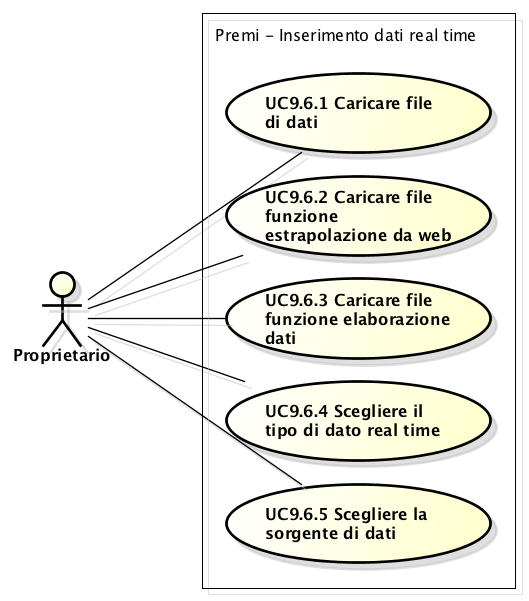
\includegraphics[scale=0.45] {img/UC9.6.png}
	\caption{UC9.6 - Inserire dati \gls{real time}} 
\end{figure}

\begin{itemize}
	\item \textbf{Attori:} Proprietario;
	\item \textbf{Scopo e descrizione:}	Un elemento di dati \gls{real time} consiste in un oggetto da inserire nella \gls{slide} che visualizzerà in modo formattato, con lo stile della presentazione, dei dati presi dall'esterno e, quindi, aggiornati al momento dell'avio della presentazione. Il programma offre delle funzioni specifiche per tipi di dato diversi che, preso in input un array di dati, lo elaborano per inserire poi i dati formattati all'interno della \gls{slide}.

	I dati contenuti nell'array devono essere salvati in modo diverso a seconda della funzione che si deve richiamare. Ogni funzione, infatti, per elaborare i dati correttamente, richiede un array con delle determinate specifiche.
	L'array di dati potrà poi essere fornito attraverso un file caricato direttamente sul server dall'utente oppure attraverso una funzione che raccoglie i dati da un sito web esterno e li ritorna all'interno di un array secondo.
	
	Le funzioni per estrapolare i dati da siti esterni e le funzioni che elaborano i dati di un array per inserire il contenuto nella \gls{slide} possono essere implementate dall'utente, il quale è così in grado di creare degli elementi specifici adatti alle situazioni di cui necessita.
	
	\item \textbf{Precondizione:} L'utente sta modificando una \gls{slide} e seleziona il comando per inserire un elemento di dati \gls{real time};
	\item \textbf{Flusso principale di eventi:}
	\begin{enumerate}
		\item L'utente carica un file contenente i dati \gls{real time} [UC9.6.1];
		\item L'utente carica un file contenente la funzione di estrapolazione dati dall'esterno [UC9.6.2];
		\item L'utente carica un file contenente la funzione di elaborazione dati dell'array [UC9.6.3];
		\item L'utente sceglie il tipo di dato \gls{real time} [UC9.6.4];
		\item L'utente sceglie i dati da inserire nella \gls{slide} [UC9.6.5].
	\end{enumerate}
	\item \textbf{Postcondizione:} Il sistema ha inserito l'elemento di dati \gls{real time} nella \gls{slide} corrente.
\end{itemize}

	\subsection{Caso d'uso UC9.6.1: Caricare un file di dati}
	\begin{itemize}
		\item \textbf{Attori:} Proprietario;
		\item \textbf{Scopo e descrizione:} L'utente deve caricare un file contenente i dati \gls{real time} nel server;
		\item \textbf{Precondizione:} L'utente ha creato un file contenente un array di dati;
		\item \textbf{Postcondizione:} Il sistema ha caricato il file nel server nella opportuna directory.
	\end{itemize}

	\subsection{Caso d'uso UC9.6.2: Caricare un file con la funzione di estrapolazione dati}
	\begin{itemize}
		\item \textbf{Attori:} Proprietario;
		\item \textbf{Scopo e descrizione:} L'utente deve caricare un file contenente la funzione di estrapolazione dei dati da un sito web. La funzione deve ritornare un array di dati;
		\item \textbf{Precondizione:} L'utente ha creato un file sorgente contenente la funzione da eseguire;
		\item \textbf{Postcondizione:} Il sistema ha caricato il file nel server nella directory dedicata a questi tipi di file.
	\end{itemize}
	
	\subsection{Caso d'uso UC9.6.3: Caricare un file con la funzione di elaborazione dati}
	\begin{itemize}
		\item \textbf{Attori:} Proprietario;
		\item \textbf{Scopo e descrizione:} L'utente deve caricare un file contenente la funzione di elaborazione dei dati dell'array passato in oggetto. La funzione deve ritornare i dati formattati per l'inserimento di essi nella \gls{slide};
		\item \textbf{Precondizione:} L'utente ha creato un file sorgente contenente la funzione da eseguire;
		\item \textbf{Postcondizione:} Il sistema ha caricato il file nel server nella directory dedicata a questi tipi di file.
	\end{itemize}
	
	\subsection{Caso d'uso UC9.6.4: Scegliere il tipo di dato real time}
	\begin{itemize}
		\item \textbf{Attori:} Proprietario;
		\item \textbf{Scopo e descrizione:} L'utente deve scegliere quale tipo di dati \gls{real time} inserire nella \gls{slide};
		\item \textbf{Precondizione:} Nel server è presente il file contenente la funzione di elaborazione dei dati;
		\item \textbf{Postcondizione:} Il sistema registra la scelta dell'utente e permette di scegliere ila sorgente di dati da inserire.
	\end{itemize}
	
	\subsection{Caso d'uso UC9.6.5: Scegliere la sorgente di dati real time da inserire}
	\begin{itemize}
		\item \textbf{Attori:} Proprietario;
		\item \textbf{Scopo e descrizione:} L'utente deve scegliere la sorgente di dati \gls{real time} da inserire nella \gls{slide}, che può essere un file contenente dei dati oppure un file avente una funzione che prenda i dati dall'esterno;
		\item \textbf{Precondizione:} Nel server è presente il file contenente la sorgente di dati compatibili con il tipo di dati \gls{real time} scelto;
		\item \textbf{Postcondizione:} Il sistema ha inserito l'oggetto di dati \gls{real time} nella \gls{slide}.
	\end{itemize}
	

\subsection{Caso d'uso UC9.7: Inserire una tabella}
\begin{itemize}
	\item \textbf{Attori:} Proprietario;
	\item \textbf{Scopo e descrizione:} L'utente deve inserire una tabella. Seleziona il numero di righe e di colonne e la inserisce nella posizione desiderata;
	\item \textbf{Precondizione:} L'utente sta modificando una \gls{slide} e seleziona il comando per inserire una tabella nella \gls{slide};
	\item \textbf{Postcondizione:} Il sistema ha inserito la tabella nella \gls{slide} corrente e attiva la modalità di modifica della tabella.
\end{itemize}


\subsection{Caso d'uso UC9.8: Inserire un grafico}
\begin{figure}[h] 
	\centering 
	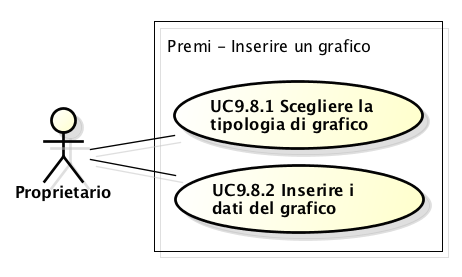
\includegraphics[scale=0.45] {img/UC9.8.png}
	\caption{UC9.8 - Inserire grafico} 
\end{figure}

\begin{itemize}
	\item \textbf{Attori:} Proprietario;
	\item \textbf{Scopo e descrizione:} L'utente deve inserire un grafico. Seleziona la tipologia del grafico tra istogramma, torta e linea, e inserisce i dati;
	\item \textbf{Precondizione:} L'utente sta modificando una \gls{slide} e seleziona il comando per inserire un grafico;
	\item \textbf{Flusso principale di eventi:}
	\begin{enumerate}
		\item L'utente sceglie la tipologia di grafico da inserire [UC9.8.1];
		\item L'utente inserisce i dati da inserire nel grafico [UC9.8.2].
	\end{enumerate}
	\item \textbf{Postcondizione:} Il sistema ha creato il grafico.
\end{itemize}

	\subsection{Caso d'uso UC9.8.1: Scegliere la tipologia del grafico}
	\begin{itemize}
		\item \textbf{Attori:} Proprietario;
		\item \textbf{Scopo e descrizione:} L'utente deve scegliere il tipo di grafico da inserire;
		\item \textbf{Precondizione:} La finestra di dialogo per la scelta del tipo di grafico è aperta;
		\item \textbf{Postcondizione:} Il sistema ha registrato la scelta dell'utente.
	\end{itemize}
	
	\subsection{Caso d'uso UC9.8.2: Inserire i dati del grafico}
	\begin{itemize}
		\item \textbf{Attori:} Proprietario;
		\item \textbf{Scopo e descrizione:} L'utente deve inserire i dati per il grafico da inserire;
		\item \textbf{Precondizione:} L'utente ha scelto il tipo di grafico;
		\item \textbf{Postcondizione:} Il sistema salva i dati inseriti.
	\end{itemize}


\subsection{Caso d'uso UC9.9: Scegliere un effetto di transizione}
\begin{itemize}
	\item \textbf{Attori:} Proprietario;
	\item \textbf{Scopo e descrizione:} L'utente deve scegliere l'effetto di transizione da dare alla \gls{slide}. Può scegliere tra scorrimento, dissolvenza, convesso, concavo e nessuno;
	\item \textbf{Precondizione:} L'utente sta modificando una presentazione e seleziona il comando per cambiare tipo di transizione tra le \gls{slide};
	\item \textbf{Postcondizione:} Il sistema ha modificato l'effetto di transizione.
\end{itemize}


\subsection{Caso d'uso UC9.10: Ridimensionamento di un elemento}
\begin{itemize}
	\item \textbf{Attori:} Proprietario;
	\item \textbf{Scopo e descrizione:} L'utente cambia la grandezza dell'elemento selezionato della \gls{slide};
	\item \textbf{Precondizione:} L'utente ha selezionato l'oggetto che vuole ridimensionare;
	\item \textbf{Postcondizione:} Il sistema ha ridimensionato l'elemento della \gls{slide} selezionato.
\end{itemize}


\subsection{Caso d'uso UC9.11: Spostamento di un elemento}
\begin{itemize}
	\item \textbf{Attori:} Proprietario;
	\item \textbf{Scopo e descrizione:} L'utente cambia la posizione dell'elemento selezionato della \gls{slide};
	\item \textbf{Precondizione:} L'utente ha selezionato l'elemento che intende spostare;
	\item \textbf{Postcondizione:} Il sistema ha spostato l'elemento della \gls{slide} selezionato.
\end{itemize}


\subsection{Caso d'uso UC9.12: Rotazione di un elemento}
\begin{itemize}
	\item \textbf{Attori:} Proprietario;
	\item \textbf{Scopo e descrizione:} L'utente ruota l'elemento selezionato della \gls{slide};
	\item \textbf{Precondizione:} L'utente ha selezionato l'oggetto che vuole ruotare;
	\item \textbf{Postcondizione:} Il sistema ha ruotato l'elemento della \gls{slide} selezionato.
\end{itemize}


\subsection{Caso d'uso UC9.13: Rimozione di un elemento}
\begin{itemize}
	\item \textbf{Attori:} Proprietario;
	\item \textbf{Scopo e descrizione:} L'utente elimina l'elemento selezionato dalla \gls{slide};
	\item \textbf{Precondizione:} L'utente ha selezionato l'oggetto che vuole rimuovere;
	\item \textbf{Postcondizione:} Il sistema ha rimosso dalla \gls{slide} l'elemento selezionato.
\end{itemize}


\subsection{Caso d'uso UC9.14: Caricamento di un file}
\begin{itemize}
	\item \textbf{Attori:} Proprietario;
	\item \textbf{Scopo e descrizione:} L'utente deve caricare un file da utilizzare nella presentazione;
	\item \textbf{Precondizione:} L'utente ha un file in locale da caricare sul server;
	\item \textbf{Postcondizione:} Il sistema ha caricato il file selezionato dall'utente e lo ha inserito nella \gls{slide}.
\end{itemize}

\newpage
\subsection{Caso d'uso UC9.15: Scegliere la formattazione del testo}
\begin{figure}[h] 
	\centering 
	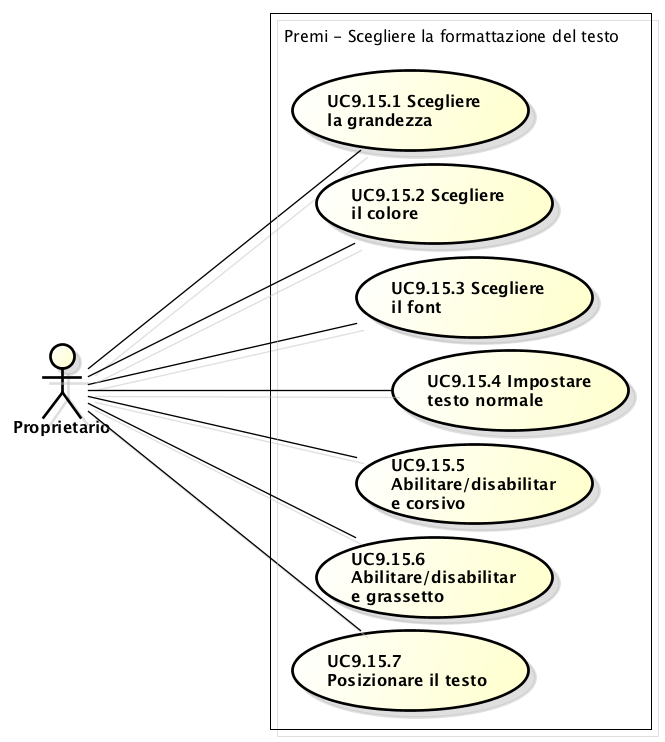
\includegraphics[scale=0.45] {img/UC9.15.png}
	\caption{UC9.15 - Scegliere la formattazione del testo}
\end{figure}

\begin{itemize}
	\item \textbf{Attori:} Proprietario;
	\item \textbf{Scopo e descrizione:} L'utente può modificare l'aspetto del testo contenuto in una casella di testo. L'utente seleziona il testo e poi sceglie che modifiche effettuare;
	\item \textbf{Precondizione:} L'utente ha selezionato un elemento di testo inserito nella \gls{slide};
	\item \textbf{Flusso principale degli eventi:}
	\begin{enumerate}
		\item L'utente può cambiare la grandezza del testo [UC9.15.1];
		\item L'utente può cambiare il colore del testo [UC9.15.2];
		\item L'utente può cambiare il \gls{font} del testo [UC9.15.3];
		\item L'utente può abilitare o disabilitare il testo in corsivo [UC9.15.4];
		\item L'utente può abilitare o disabilitare il testo in grassetto [UC9.15.5];
		\item L'utente può spostare il testo in una nuova posizione [UC9.15.6].
	\end{enumerate}
	\item \textbf{Postcondizione:} Il sistema ha apportato le modifiche scelte all'elemento di testo selezionato.
\end{itemize}

\subsection{Caso d'uso UC9.15.1: Scegliere la grandezza}
\begin{itemize}
	\item \textbf{Attori:} Proprietario;
	\item \textbf{Scopo e descrizione:} L'utente può cambiare la grandezza del testo;
	\item \textbf{Precondizione:} Il testo da modificare è selezionato;
	\item \textbf{Postcondizione:} Il testo è stato ingrandito o rimpicciolito secondo la scelta dell'utente.
\end{itemize}

\subsection{Caso d'uso UC9.15.2: Scegliere il colore}
\begin{itemize}
	\item \textbf{Attori:} Proprietario;
	\item \textbf{Scopo e descrizione:} L'utente può cambiare il colore del testo;
	\item \textbf{Precondizione:} Il testo da modificare è selezionato;
	\item \textbf{Postcondizione:} Il testo è stato colorato secondo la scelta dell'utente.
\end{itemize}

\subsection{Caso d'uso UC9.15.3: Scegliere il font}
\begin{itemize}
	\item \textbf{Attori:} Proprietario;
	\item \textbf{Scopo e descrizione:} L'utente può cambiare il \gls{font} del testo;
	\item \textbf{Precondizione:} Il testo da modificare è selezionato;
	\item \textbf{Postcondizione:} Il testo ha cambiato \gls{font} secondo la scelta dell'utente.
\end{itemize}

\subsection{Caso d'uso UC9.15.4: Abilitare/disabilitare corsivo}
\begin{itemize}
	\item \textbf{Attori:} Proprietario;
	\item \textbf{Scopo e descrizione:} L'utente può abilitare o disabilitare la scrittura in corsivo;
	\item \textbf{Precondizione:} Il testo da modificare è selezionato;
	\item \textbf{Postcondizione:} Il testo è stato modificato secondo la scelta dell'utente.
\end{itemize}

\subsection{Caso d'uso UC9.15.5: Abilitare/Disabilitare grassetto}
\begin{itemize}
	\item \textbf{Attori:} Proprietario;
	\item \textbf{Scopo e descrizione:} L'utente può abilitare o disabilitare la scrittura in grassetto;
	\item \textbf{Precondizione:} Il testo da modificare è selezionato;
	\item \textbf{Postcondizione:} Il testo è stato modificato secondo la scelta dell'utente.
\end{itemize}

\subsection{Caso d'uso UC9.15.6: Posizionare il testo}
\begin{itemize}
	\item \textbf{Attori:} Proprietario;
	\item \textbf{Scopo e descrizione:} L'utente può allineare il testo in una nuova posizione;
	\item \textbf{Precondizione:} Il testo da modificare è selezionato;
	\item \textbf{Postcondizione:} Il testo è stata allineato secondo la scelta dell'utente.
\end{itemize}

\newpage
\subsection{Caso d'uso UC9.16: Modificare una tabella}
\begin{figure}[h] 
	\centering 
	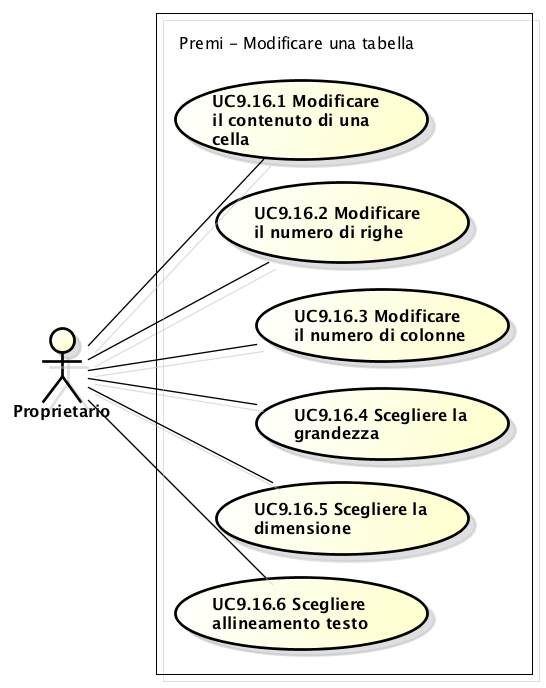
\includegraphics[scale=0.45] {img/UC9.16.png}
	\caption{UC9.16 - Modificare una tabella}
\end{figure}

\begin{itemize}
	\item \textbf{Attori:} Proprietario;
	\item \textbf{Scopo e descrizione:} L'utente può modificare l'aspetto della tabella e del suo contenuto. L'utente seleziona la tabella o il testo e poi sceglie che modifiche effettuare;
	\item \textbf{Precondizione:} L'utente ha selezionato una tabella, o una parte di essa, già inserita nella \gls{slide};
	\item \textbf{Flusso principale degli eventi:}
	\begin{enumerate}
		\item L'utente può modificare il contenuto di una cella [UC9.16.1];
		\item L'utente può modificare il numero di righe [UC9.16.2];
		\item L'utente può modificare il numero di colonne [UC9.16.3];
		\item L'utente può cambiare la grandezza della tabella [UC9.16.4];
		\item L'utente può cambiare il colore di sfondo della tabella [UC9.16.5];
		\item L'utente può cambiare l'allineamento del testo [UC9.16.6].
	\end{enumerate}
	\item \textbf{Postcondizione:} Il sistema ha apportato le modifiche scelte alla tabella.
\end{itemize}

	\subsection{Caso d'uso UC9.16.1: Modificare il contenuto di una cella della tabella}
	\begin{itemize}
		\item \textbf{Attori:} Proprietario;
		\item \textbf{Scopo e descrizione:} L'utente può modificare il contenuto di una cella della tabella, cioè aggiungere e modificare elementi di testo;
		\item \textbf{Precondizione:} La cella da modificare è stata selezionata;
		\item \textbf{Postcondizione:} Il contenuto della cella è stato modificato.
	\end{itemize}
	
	\subsection{Caso d'uso UC9.16.2: Modificare il numero di righe della tabella}
	\begin{itemize}
		\item \textbf{Attori:} Proprietario;
		\item \textbf{Scopo e descrizione:} L'utente può modificare il numero di righe della tabella;
		\item \textbf{Precondizione:} L'utente ha selezionato la tabella da modificare;
		\item \textbf{Postcondizione:} La tabella è stata modificata nelle sue dimensioni secondo il numero di righe scelto dell'utente.
	\end{itemize}
	
	\subsection{Caso d'uso UC9.16.3: Modificare il numero di colonne della tabella}
	\begin{itemize}
		\item \textbf{Attori:} Proprietario;
		\item \textbf{Scopo e descrizione:} L'utente può modificare il numero di colonne della tabella;
		\item \textbf{Precondizione:} L'utente ha selezionato la tabella da modificare;
		\item \textbf{Postcondizione:} La tabella è stata modificata nelle sue dimensioni secondo il numero di colonne scelto dell'utente.
	\end{itemize}
	
	\subsection{Caso d'uso UC9.16.4: Scegliere grandezza della tabella}
	\begin{itemize}
		\item \textbf{Attori:} Proprietario;
		\item \textbf{Scopo e descrizione:} L'utente può modificare la grandezza della tabella;
		\item \textbf{Precondizione:} L'utente ha selezionato la tabella da modificare;
		\item \textbf{Postcondizione:} La tabella è stata modificata nelle sue dimensioni secondo la scelta dell'utente.
	\end{itemize}
	
	\subsection{Caso d'uso UC9.16.5: Scegliere colore di sfondo della tabella}
	\begin{itemize}
		\item \textbf{Attori:} Proprietario;
		\item \textbf{Scopo e descrizione:} L'utente può modificare il colore di sfondo della tabella;
		\item \textbf{Precondizione:} La tabella o le celle da modificare sono state selezionate;
		\item \textbf{Postcondizione:} Lo sfondo della tabella o delle celle è stato modificato secondo la scelta dell'utente.
	\end{itemize}
	
	\subsection{Caso d'uso UC9.16.6: Scegliere allineamento del testo}
	\begin{itemize}
		\item \textbf{Attori:} Proprietario;
		\item \textbf{Scopo e descrizione:} L'utente può modificare l'allineamento del testo della tabella;
		\item \textbf{Precondizione:} La tabella o le celle da modificare sono state selezionate;
		\item \textbf{Postcondizione:} L'allineamento del testo della tabella o delle celle è stato modificato secondo la scelta dell'utente.
	\end{itemize}
	
	
	\subsection{Caso d'uso UC9.17: Personalizzare un grafico}
	\begin{figure}[h] 
		\centering 
		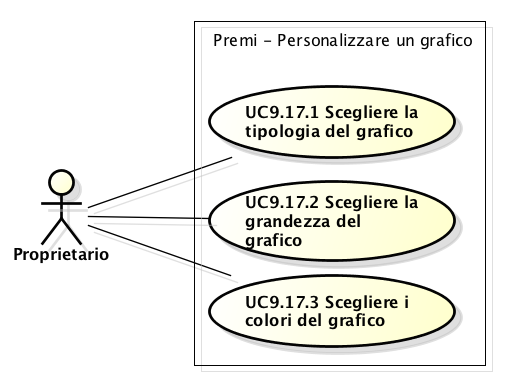
\includegraphics[scale=0.45] {img/UC9.17.png}
		\caption{UC9.17 - Personalizzare un grafico} 
	\end{figure}
	
	\begin{itemize}
		\item \textbf{Attori:} Proprietario;
		\item \textbf{Scopo e descrizione:} L'utente può modificare la tipologia e l'aspetto del grafico. L'utente seleziona il grafico e poi sceglie che modifiche effettuare;
		\item \textbf{Precondizione:} L'utente ha selezionato un grafico già inserito in una \gls{slide};
		\item \textbf{Flusso principale degli eventi:}
		\begin{enumerate}
			\item L'utente può cambiare la tipologia del grafico [UC9.17.1];
			\item L'utente può cambiare la dimensione del grafico [UC9.17.2];
			\item L'utente può cambiare i colori del grafico [UC9.17.3].
		\end{enumerate}
		\item \textbf{Postcondizione:} Il sistema ha apportato le modifiche scelte al grafico.
	\end{itemize}

		\subsection{Caso d'uso UC9.17.1: Scegliere la tipologia del grafico}
		\begin{itemize}
			\item \textbf{Attori:} Proprietario;
			\item \textbf{Scopo e descrizione:} L'utente deve modificare la tipologia del grafico. Seleziona il grafico e il comando per cambiare il tipo;
			\item \textbf{Precondizione:} L'utente ha selezionato il grafico da modificare;
			\item \textbf{Postcondizione:} La tipologia del grafico è stata modificata secondo la scelta dell'utente.
		\end{itemize}
		
		\subsection{Caso d'uso UC9.17.2: Scegliere la grandezza del grafico}
		\begin{itemize}
			\item \textbf{Attori:} Proprietario;
			\item \textbf{Scopo e descrizione:} L'utente deve modificare la grandezza del grafico;
			\item \textbf{Precondizione:} L'utente ha selezionato il grafico da modificare;
			\item \textbf{Postcondizione:} Il grafico è stato modificato nelle sue dimensioni secondo la scelta dell'utente.
		\end{itemize}
		
		\subsection{Caso d'uso UC9.17.3: Scegliere i colori del grafico}
		\begin{itemize}
			\item \textbf{Attori:} Proprietario;
			\item \textbf{Scopo e descrizione:} L'utente deve modificare il set di colori del grafico;
			\item \textbf{Precondizione:} L'utente ha selezionato il grafico da modificare;
			\item \textbf{Postcondizione:} I colori del grafico sono stati modificati secondo la scelta dell'utente.
		\end{itemize}


\subsection{Caso d'uso UC9.18: Inserire note/parole chiave}
\begin{itemize}
	\item \textbf{Attori:} Proprietario;
	\item \textbf{Scopo e descrizione:} L'utente deve inserire delle note o delle parole chiave nella \gls{slide} da usare durante la visualizzazione della presentazione in modalità presentatore. Seleziona il comando e inserisce ciò che desidera includere;
	\item \textbf{Precondizione:} L'utente sta modificando una \gls{slide} e seleziona il comando per inserire le note/parole chiave;
	\item \textbf{Postcondizione:} Il sistema inserisce le note/parole chiave che l'utente ha aggiunto nella \gls{slide} corrente.
\end{itemize}

\subsection{Caso d'uso UC9.19: Spostare una slide}
\begin{itemize}
	\item \textbf{Attori:} Proprietario;
	\item \textbf{Scopo e descrizione:} L'utente vuole spostare una \gls{slide} della presentazione precedentemente creata in un'altra posizione. Usa quindi gli appositi pulsanti per spostarla tra le slide nella posizione desiderata.
	\item \textbf{Precondizione:} L'utente è nella schermata di visualizzazione globale della presentazione è ha creato almeno due slide;
	\item \textbf{Postcondizione:} La \gls{slide} è stata spostata.
\end{itemize}
